\documentclass[11pt,a4paper,twoside]{article}
\usepackage{lmodern}
\usepackage{amssymb,amsmath}
\usepackage{ifxetex,ifluatex}
\usepackage{fixltx2e} % provides \textsubscript
\ifnum 0\ifxetex 1\fi\ifluatex 1\fi=0 % if pdftex
  \usepackage[T1]{fontenc}
  \usepackage[utf8]{inputenc}
\else % if luatex or xelatex
  \ifxetex
    \usepackage{mathspec}
  \else
    \usepackage{fontspec}
  \fi
  \defaultfontfeatures{Ligatures=TeX,Scale=MatchLowercase}
\fi
% use upquote if available, for straight quotes in verbatim environments
\IfFileExists{upquote.sty}{\usepackage{upquote}}{}
% use microtype if available
\IfFileExists{microtype.sty}{%
\usepackage{microtype}
\UseMicrotypeSet[protrusion]{basicmath} % disable protrusion for tt fonts
}{}
\usepackage[left=2.5cm,right=3.5cm,top=83.75pt,textheight=24.35cm,textwidth=15cm,a4paper,headheight=13.6pt,twoside=true]{geometry}
\usepackage{hyperref}
\hypersetup{unicode=true,
            pdfborder={0 0 0},
            breaklinks=true}
\urlstyle{same}  % don't use monospace font for urls
\usepackage{biblatex}

\addbibresource{literatur.bib}
\addbibresource{packages.bib}
\usepackage{longtable,booktabs}
\usepackage{graphicx,grffile}
\makeatletter
\def\maxwidth{\ifdim\Gin@nat@width>\linewidth\linewidth\else\Gin@nat@width\fi}
\def\maxheight{\ifdim\Gin@nat@height>\textheight\textheight\else\Gin@nat@height\fi}
\makeatother
% Scale images if necessary, so that they will not overflow the page
% margins by default, and it is still possible to overwrite the defaults
% using explicit options in \includegraphics[width, height, ...]{}
\setkeys{Gin}{width=\maxwidth,height=\maxheight,keepaspectratio}
\IfFileExists{parskip.sty}{%
\usepackage{parskip}
}{% else
\setlength{\parindent}{0pt}
\setlength{\parskip}{6pt plus 2pt minus 1pt}
}
\setlength{\emergencystretch}{3em}  % prevent overfull lines
\providecommand{\tightlist}{%
  \setlength{\itemsep}{0pt}\setlength{\parskip}{0pt}}
\setcounter{secnumdepth}{5}
% Redefines (sub)paragraphs to behave more like sections
\ifx\paragraph\undefined\else
\let\oldparagraph\paragraph
\renewcommand{\paragraph}[1]{\oldparagraph{#1}\mbox{}}
\fi
\ifx\subparagraph\undefined\else
\let\oldsubparagraph\subparagraph
\renewcommand{\subparagraph}[1]{\oldsubparagraph{#1}\mbox{}}
\fi

%%% Use protect on footnotes to avoid problems with footnotes in titles
\let\rmarkdownfootnote\footnote%
\def\footnote{\protect\rmarkdownfootnote}

%%% Change title format to be more compact
\usepackage{titling}

% Create subtitle command for use in maketitle
\newcommand{\subtitle}[1]{
  \posttitle{
    \begin{center}\large#1\end{center}
    }
}

\setlength{\droptitle}{-2em}

  \title{}
    \pretitle{\vspace{\droptitle}}
  \posttitle{}
    \author{}
    \preauthor{}\postauthor{}
    \date{}
    \predate{}\postdate{}
  
\usepackage{booktabs}
\usepackage[ngerman,english]{babel} % deutsche Trennregeln, "Inhaltsverzeichnis" etc.
\usepackage{mathptmx} % Times-Roman-Schrift (auch für mathematische Formeln)
\usepackage{pdfpages}
\usepackage{pgf}
\usepackage{epstopdf}

\usepackage{caption}
\usepackage{changepage}
\usepackage{subcaption}
\usepackage{hanging}

% custom imports
% multirows für Tabellen
\usepackage{multirow}
% nice quotes
\usepackage[autostyle=true,german=quotes]{csquotes}

\usepackage[onehalfspacing]{setspace} % 1,5facher Zeilenabstand

% Zum Setzen von URLs
\usepackage{color}
\definecolor{darkred}{rgb}{0.25,0,0}
\definecolor{darkgreen}{rgb}{0,0.2,0}
\definecolor{darkmagenta}{rgb}{0.2,0,0.2}
\definecolor{darkcyan}{rgb}{0,0.15,0.15}

\usepackage{fancyhdr} % Positionierung der Seitenzahlen

\renewcommand{\headrulewidth}{0pt}

% Korrektes Format für Nummerierung von Abbildungen (figure) und
% Tabellen (table): <Kapitelnummer>.<Abbildungsnummer>
\makeatletter
\@addtoreset{figure}{section}
\renewcommand{\thefigure}{\thesection.\arabic{figure}}
\@addtoreset{table}{section}
\renewcommand{\thetable}{\thesection.\arabic{table}}
\makeatother

%\sloppy % Damit LaTeX nicht so viel über "overfull hbox" u.Ä. meckert

% römische numerale für Inhaltsverzeichnis; wird in index.Rmd zurückgesetzt
\fancyhead[LE,RO,LO,RE]{}
\fancyfoot[CE,CO,RE,LO]{}
\fancyfoot[LE,RO]{\roman{page}}

\begin{document}

\pagestyle{empty} % Vorerst keine Seitenzahlen
\pagenumbering{alph} % Unsichtbare alphabetische Nummerierung

\begin{center}
\textsc{Ludwig-Maximilians-Universität München}\\
Department ``Institut für Informatik''\\
Professur für Computational Social Science and Big Data\\
Prof.\ Jürgen Pfeffer

\vspace{4.75cm}
{\large\textbf{Masterarbeit}}\vspace{.5cm}

{\Huge{}Not all those who wander are lost}\\\vspace{.5cm}
{\Large{}Dynamiken bei der Interessensentwicklung in Online Communities}\vspace{.75cm}

{\large Oliver Baumann}\\\href{mailto:baumanno@cip.ifi.lmu.de}{<baumanno@cip.ifi.lmu.de>}

\end{center}
\vfill

\begin{tabular}{ll}
Bearbeitungszeitraum: & 30.04.2018 bis 29.10.2018\\
Betreuer: & Dr.\ Mirco Schönfeld\\
Verantw. Hochschullehrer: & Prof.\ Jürgen Pfeffer
\end{tabular}

%______________________________________________________________________

\clearpage
\section*{Zusammenfassung}

Die vorliegende Arbeit reiht sich in Forschungsliteratur zu interaktiven Tischen, interaktiven Arbeitsumgebungen,
gekrümmten Multitouch-Displays und indirekten Multitouch-Mappings ein. Anhand einer Nutzerstudie wird die Wirkung zweier indirekter
Eingabemodi auf den Nutzer untersucht. Dazu wurde für \emph{Curve}, ein interaktiver Tisch mit gebogenem Display,
eine prototypische Anwendung entwickelt, die entweder mit einer Maus oder über Multitouch-Gesten bedient werden kann.
Im Gegensatz zu isolierten Tasks ermöglicht die Anwendung den von einer Desktopumgebung gewohnten Arbeitsablauf. Das System
bietet für den Anwendungsfall "`Audio-Bearbeitung"' die Möglichkeit, in einem Audio-Sample zu navigieren und dieses
zu modifizieren. Die beiden Interface-Varianten wurden auf ihre Wirkung auf das Nutzererlebnis und ihre Eignung
zum Einsatz in interaktiven Arbeitsplätzen hin untersucht. Es wurde festgestellt, dass keine der beiden Varianten
dabei übermäßig gut oder schlecht abschneidet. Beide Eingabetechniken sind dabei ähnlich gut für den speziellen
Anwendungsfall geeignet. Ein Transfer zu anderen Einsatzmöglichkeiten schließt die Arbeit ab. Es sei darauf hingewiesen,
dass die in dieser Studie präsentierten Ergebnisse anhand einer kleinen Stichprobe ermittelt wurden und möglicherweise
nicht vollends generalisierbar sind.

\iffalse
\selectlanguage{english}
\section*{Abstract}

We relate in parts to previous work on interactive desks, interactive workspaces, bent multitouch-enabled displays
and indirect mappings for multitouch. Based on a user-study, we compare the effects of two interaction techniques on the user.
To this end, we implemented a prototypical application for \emph{Curve}, an interactive desk with a bent multitouch-display.
The user can interact with the application either via a mouse, or via multitouch-gestures.
In contrast to isolated tasks commonly used, our system enables a workflow comparable to that of a traditional desktop
environment. The system relates to the specific use-case of audio-editing and allows for navigating and manipulating an audio-sample.
Both interaction techniques presented here have been studied with regard to their effect on user experience and their
compatibility with being used in interactive workspaces. We conclude that neither of the two techniques out- or underperforms
and thus suggest that they are equally suitable for this particular use case. We end with suggesting other possible applications
of this setup, not restricted to any single use-case. We note, however, that due to the small sample size of our study, the
findings presented here might not be fully generalizable.
\selectlanguage{ngerman}
\fi
\clearpage
\section*{Aufgabenstellung}

\selectlanguage{english}
Lorem ipsum

\vfill % Sorgt dafür, dass das Folgende an das Seitenende rutscht

\selectlanguage{ngerman}

\noindent Ich erkläre hiermit, dass ich die vorliegende Arbeit
selbstständig angefertigt, alle Zitate als solche kenntlich gemacht
sowie alle benutzten Quellen und Hilfsmittel angegeben habe.

\bigskip\noindent München, \today

\vspace{4ex}\noindent\makebox[7cm]{\dotfill}

%______________________________________________________________________

\cleardoublepage


%Abbildungsverzeichnis erzeugen - normalerweise nicht nötig
%\cleardoublepage
%\listoffigures
%______________________________________________________________________

\cleardoublepage



\pagestyle{fancy}
\pagenumbering{roman} % Römische Seitenzahlen
\setcounter{page}{1}

{
\setcounter{tocdepth}{3}
\tableofcontents
}
\cleardoublepage

\pagenumbering{arabic}
\setcounter{page}{1}

\fancyhead[LE,RO]{\rightmark}
\fancyhead[LO,RE]{\leftmark}
\fancyfoot[LE,RO]{\thepage}

\cleardoublepage

\hypertarget{einleitung}{%
\section{Einleitung}\label{einleitung}}

\cleardoublepage

\hypertarget{grundlagen-und-verwandte-forschung}{%
\section{Grundlagen und verwandte
Forschung}\label{grundlagen-und-verwandte-forschung}}

\hypertarget{topic-modelle}{%
\subsection{Topic-Modelle}\label{topic-modelle}}

\hypertarget{lda}{%
\subsubsection{LDA}\label{lda}}

\hypertarget{verwandte-arbeiten}{%
\subsubsection{Verwandte Arbeiten}\label{verwandte-arbeiten}}

\hypertarget{soziale-netzwerkanalyse}{%
\subsection{Soziale Netzwerkanalyse}\label{soziale-netzwerkanalyse}}

\hypertarget{graphen-und-netzwerke}{%
\subsubsection{Graphen und Netzwerke}\label{graphen-und-netzwerke}}

\hypertarget{ego-netzwerke}{%
\subsubsection{Ego-Netzwerke}\label{ego-netzwerke}}

\hypertarget{verwandte-arbeiten-1}{%
\subsubsection{Verwandte Arbeiten}\label{verwandte-arbeiten-1}}

\hypertarget{reddit}{%
\subsection{Reddit}\label{reddit}}

\hypertarget{begriffsklarung}{%
\subsubsection{Begriffsklärung}\label{begriffsklarung}}

\hypertarget{verwandte-arbeiten-2}{%
\subsubsection{Verwandte Arbeiten}\label{verwandte-arbeiten-2}}

\cleardoublepage

\hypertarget{datenanalyse}{%
\section{Datenanalyse}\label{datenanalyse}}

\hypertarget{methodik}{%
\subsection{Methodik}\label{methodik}}

\hypertarget{datensatz}{%
\subsubsection{Datensatz}\label{datensatz}}

\hypertarget{coherence}{%
\paragraph{Kohärenz der Daten}\label{coherence}}

Im März 2018 haben Gaffney und
Matias\textasciitilde{}\autocite{Gaffney2018} eine umfassende Analyse
des Baumgartner-Korpus unternommen. Sie kommen zu dem Schluss, dass
sowohl die Erfassung der Beiträge (\emph{submissions}) als auch der
Kommentare (\emph{comments}) Lücken aufweist, also Elemente gänzlich
nicht vorhanden sind.

Da jedes Datum auf Reddit, Beiträge wie Kommentare, eine eindeutige
numerische ID besitzt, nimmt Baumgartners System Blöcke von jeweils 100
solcher Identifikatoren und stellt zu jedem davon eine Anfrage an die
Reddit-API\textasciitilde{}\autocite{Baumgartner2018a}. Da Reddit auch
auf Anfragen nach gelöschten Elementen mit einem sinnvollen Objekt
antwortet, insbesondere aber nicht mit einer Fehlermeldung, sollte
dieser Bereich von 100 sequentiellen IDs vollständig im Datensatz
abgebildet sein, inklusive als gelöscht markierte Elemente. Gaffney und
Matias machen jedoch für den Zeitraum Dezember 2005 bis Februar 2016
943.755 fehlende Kommentar- und 1.539.583 fehlende Beitrags-IDs aus.




\begin{figure}

{\centering 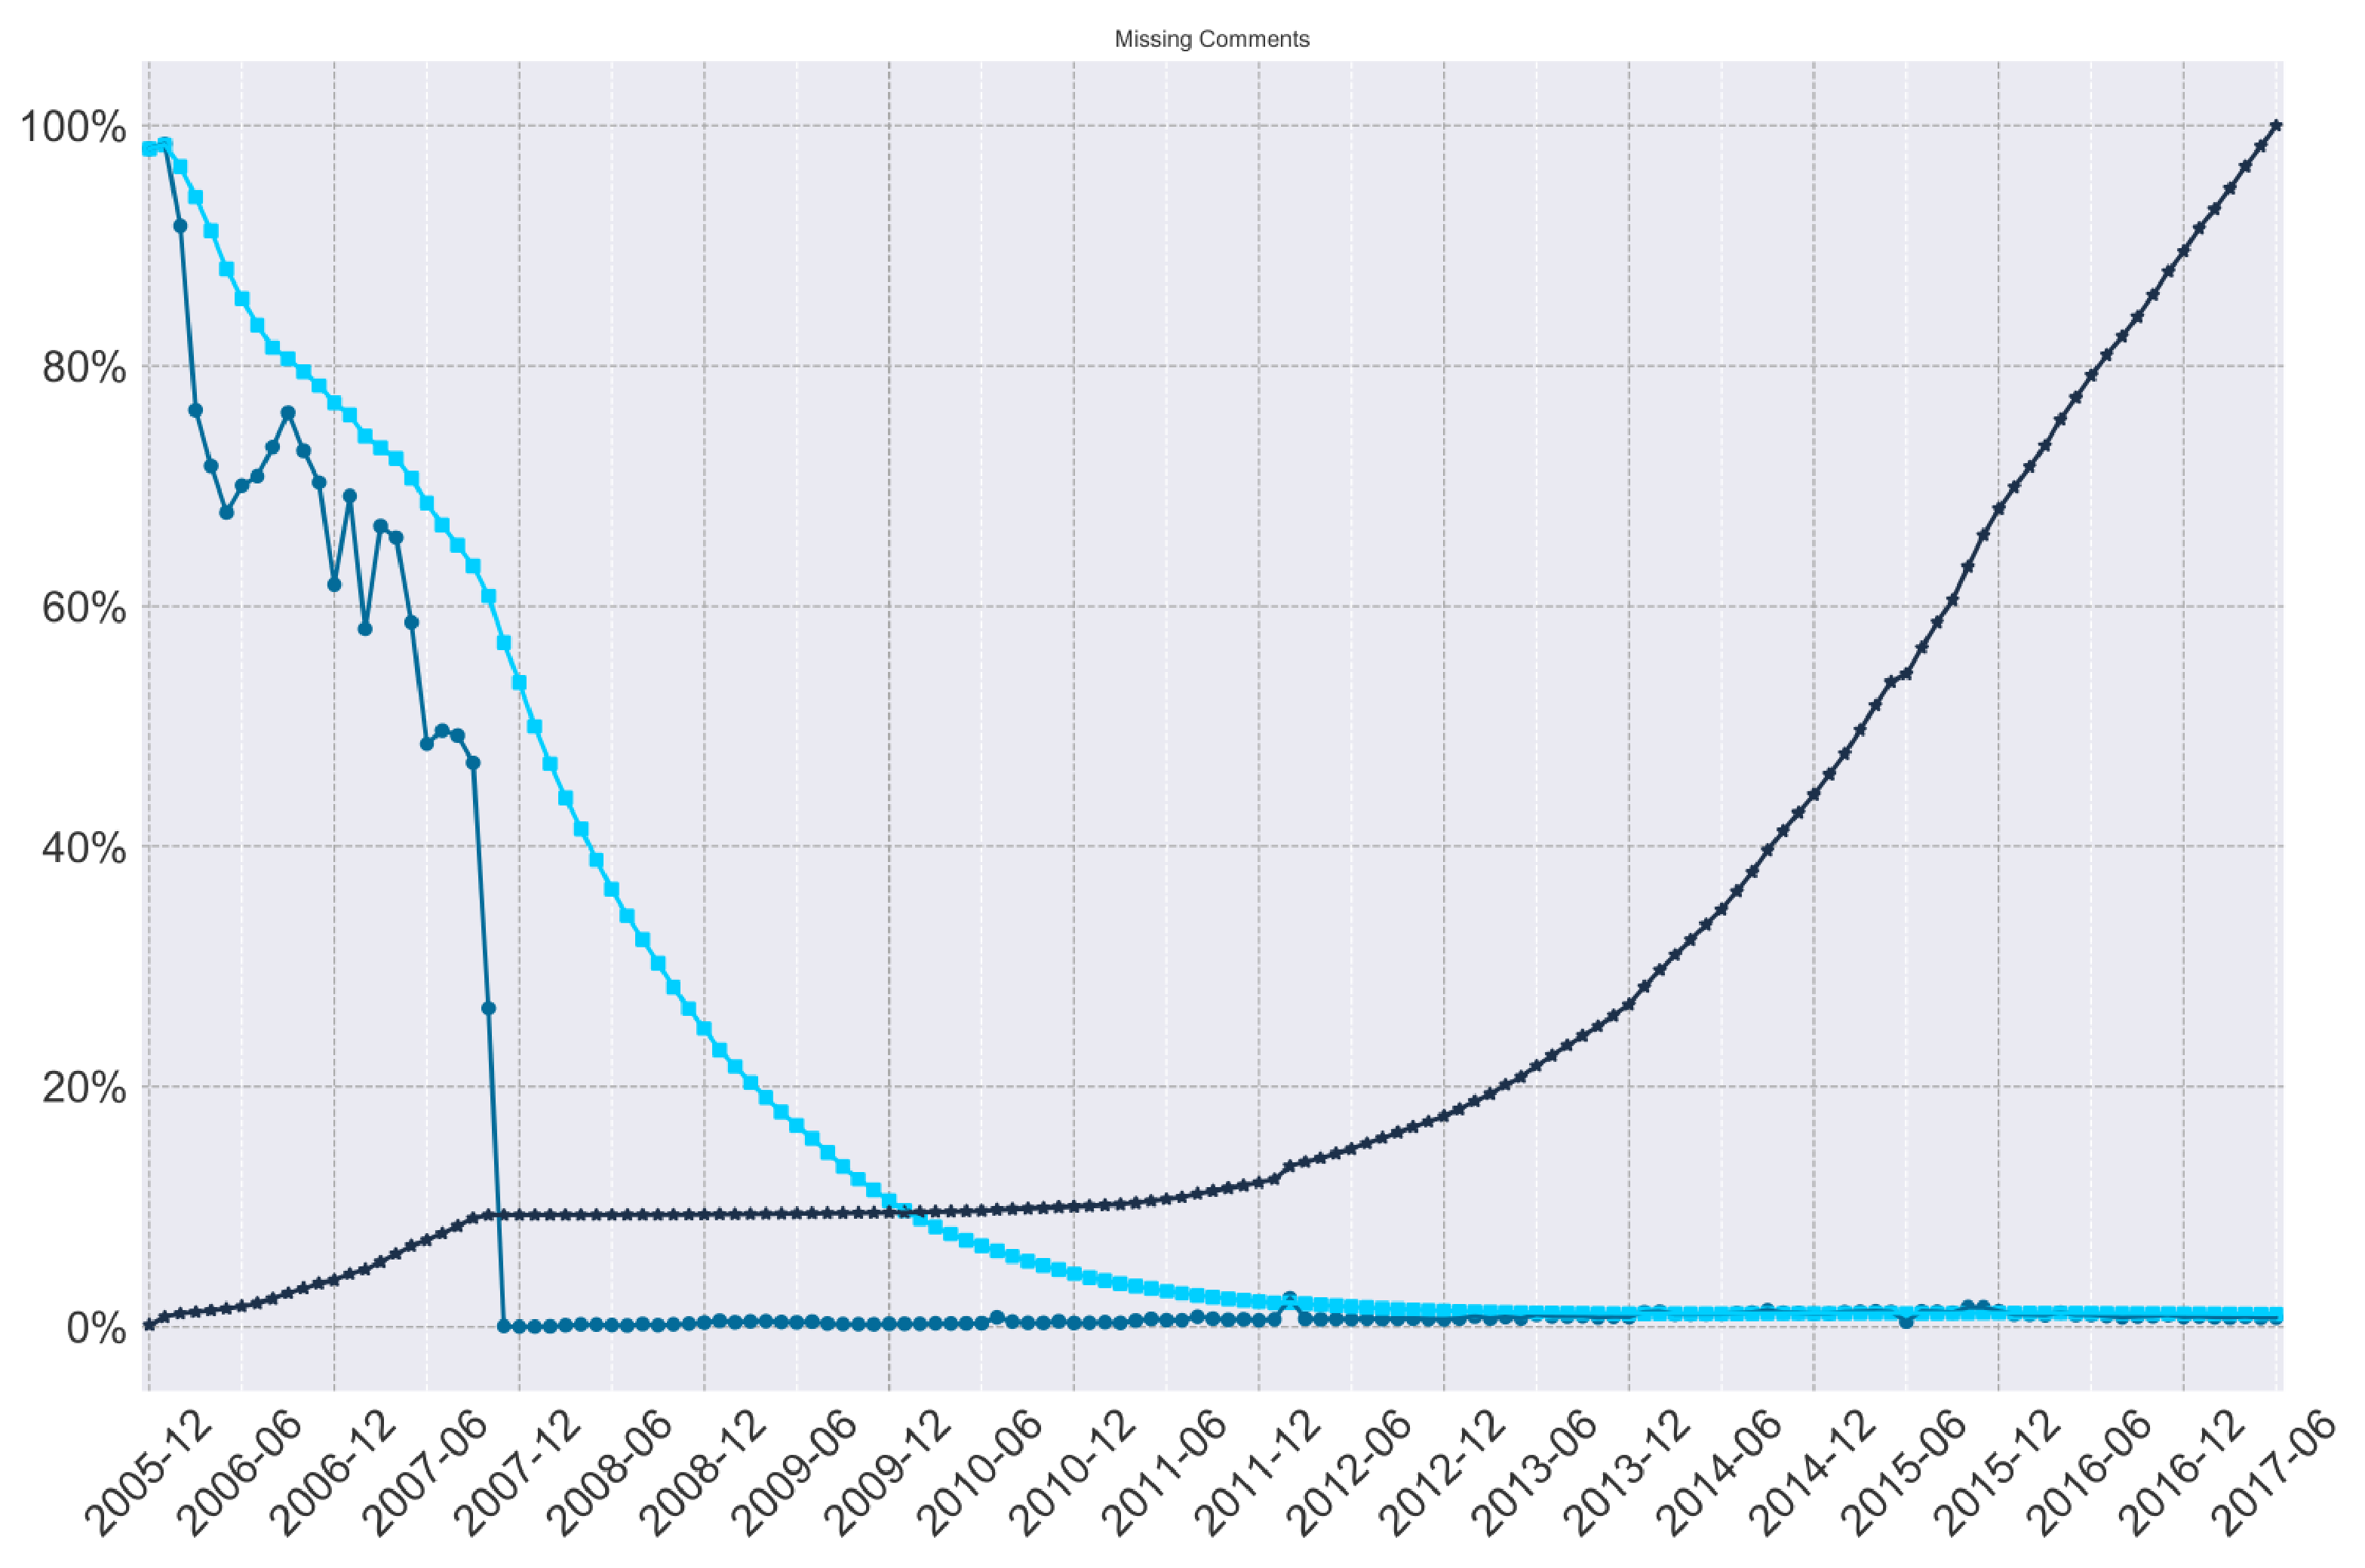
\includegraphics[width=0.8\linewidth]{./images/gaffneymatias_fig4} 

}

\caption{Verschiedene Maße zur Bestimmung fehlender Kommentare
\autocite{Gaffney2018}}\label{fig:gf4}
\end{figure}

Die mittelblauen Punkte (bis Juni 2007 die \enquote{mittlere} der drei
Linien) in Abbildung \ref{fig:gf4} zeigen den prozentualen Anteil
fehlender Einträge an der Gesamtzahl aller Kommentare für einen Monat.
Ab August 2007 fällt diese Linie stark ab und stabilisiert sich ab
November 2007 im niedrigen einstelligen Bereich, was darauf hindeutet,
dass ab diesem Zeitpunkt die Erhebung der Kommentare nahezu vollständig
verläuft und kaum noch Lücken aufweist. Obgleich die fehlenden
Kommentardaten in der Folge der Veröffentlichung von Gaffney und Matias
nachgepflegt werden\textasciitilde{}\autocite{Baumgartner2018} wird sich
die vorliegende Analyse auf den Zeitraum beginnend mit November 2007 bis
April 2018 beschränken.

\hypertarget{ergebnisse}{%
\subsection{Ergebnisse}\label{ergebnisse}}

\cleardoublepage

\hypertarget{diskussion}{%
\section{Diskussion}\label{diskussion}}

\cleardoublepage

\hypertarget{zusammenfassung-und-ausblick}{%
\section{Zusammenfassung und
Ausblick}\label{zusammenfassung-und-ausblick}}

\printbibliography


\end{document}
